\chapter{Как читать численные результаты}
\label{exp:chapter}

В опыте \texttt{low} модель SVD-SNO v2 предсказывает рассеянное
поле в эталонной среде GMsFEM. На 216 тестовых запросах средняя
ошибка рассеянного поля составляет $0{,}7575\%$ относительно
эталонного решения методом конечных элементов (FEM).

\section{Задача, эталон и тестовые запросы}

Область $(-2,2)^2$ содержит 24 круговых включения. В фоне $A=n=1$,
во включениях $A=0{,}2$ и $n=10$. Для запроса $(k,\theta)$
систему~\eqref{math:fem-system} решают на P1-элементах исходной сетки
\path{gmsfem/meshes/reference_n20_h0p04.msh}. Её целевой шаг
$h=0{,}02$, число узлов $53\,246$, число треугольников $105\,690$.
Сохранены координаты, связность и порядок узлов эталона GMsFEM.
При $k=1$, $\theta=0$ повторный расчёт воспроизвёл эталонное поле
с относительным расхождением $9{,}1\cdot10^{-14}$.

К 160 значениям $k$, равномерно распределённым на $[0{,}1;2]$,
добавили $k=1$. Для каждой частоты взяли восемь направлений с шагом
$\pi/4$; начальный угол задан псевдослучайно, при $k=1$ он равен нулю.
Все восемь полей одной частоты попадают в одну выборку.
Группы $k=0{,}1$, $1$ и $2$ заранее отложены для теста.

\begin{table}[htbp]
\centering
\caption{Разбиение 1288 полей по частотам в опыте \texttt{low}.}
\label{exp:split}
\begin{tabular}{@{}lrrr@{}}
\toprule
 & Обучение & Валидация & Итоговый тест\\
\midrule
Значений $k$ & 107 & 27 & 27\\
Комплексных полей & 856 & 216 & 216\\
\bottomrule
\end{tabular}
\end{table}

При фиксированной среде входные POD-ранги $A$ и $n$ равны нулю.
Базисы и нормировки построены по обучающим полям. На валидации
выбраны выходной ранг и эпоха для сохранения весов. Тест проверяет
прогнозы для отложенных частот и направлений той же среды,
включая обе границы диапазона.

Для тестового запроса $q$ относительная ошибка рассеянного поля равна
\begin{equation}
 e_q=100\,\frac{\norm{\widehat u_{s,q}-u_{s,h,q}}_M}
                       {\norm{u_{s,h,q}}_M}\ \%,\qquad
 \norm{v}_M=\sqrt{v^*Mv}.
 \label{exp:metric}
\end{equation}
Матрица $M$ --- согласованная матрица масс эталонной сетки. Она
учитывает обе компоненты комплексной разности и даёт $L^2$-норму
кусочно-линейного поля.

\begin{table}[htbp]
\centering
\caption{Относительная комплексная ошибка рассеянного поля на
216 тестовых запросах. Среднее взято с одинаковым весом по запросам.}
\label{exp:stats}
\begin{tabular}{@{}rrrr@{}}
\toprule
Среднее & Медиана & 95-й процентиль & Максимум\\
\midrule
$0{,}7575\%$ & $0{,}3924\%$ & $2{,}6427\%$ & $6{,}0003\%$\\
\bottomrule
\end{tabular}
\end{table}

Около половины тестовых ошибок лежат ниже $0{,}3924\%$,
а около $95\%$ --- ниже $2{,}6427\%$. На отдельных запросах
отклонение от эталона достигает примерно $6\%$.

\clearpage
\section{Что сохраняют 25 мод в каждой компоненте}

По обучающим снимкам построены два вещественных POD-базиса,
отдельно для $\operatorname{Re}u_{s,h}$ и $\operatorname{Im}u_{s,h}$.
Использована рандомизированная SVD с диагональными весами узлов
$W=\diag(M\bm1)$. Перебор шёл до 96 мод на канал. Ранг 25 первым
достиг порога $0{,}1\%$ для средней ошибки проекции на валидации
по критерию~\eqref{code:rank-criterion}. Коэффициенты при этом
вычисляются с весами $W$, а ошибка измеряется в норме $M$.
В каждом канале декодер имеет вид $\mu+\sum_{j=1}^{25}a_j\phi_j$.

\begin{figure}[htbp]
\centering
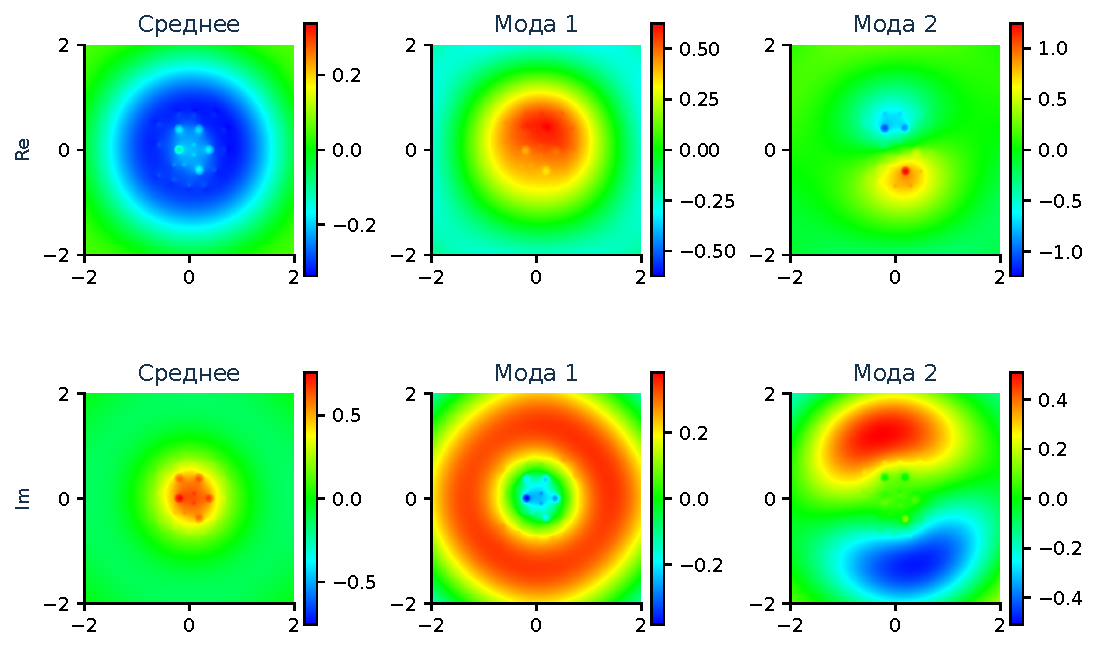
\includegraphics[width=.78\textwidth]{assets/pod_modes.pdf}
\caption{Обучающее среднее и первые две моды. Верхний ряд
соответствует вещественной части рассеянного поля, нижний --- мнимой.
У каждой карты своя шкала.}
\label{exp:modes}
\end{figure}

На верхней средней карте рисунка~\ref{exp:modes} изображена
$\phi_1$ вещественной части. Если увеличить её коэффициент на
$\delta>0$, поле в точке $x$ изменится на $\delta\phi_1(x)$.
Там, где мода жёлтая или красная, поле возрастёт, а где голубая или синяя,
уменьшится. Зелёный соответствует нулю. Смена знаков
у моды и её коэффициента сохраняет восстановленное поле.

\begin{figure}[htbp]
\centering
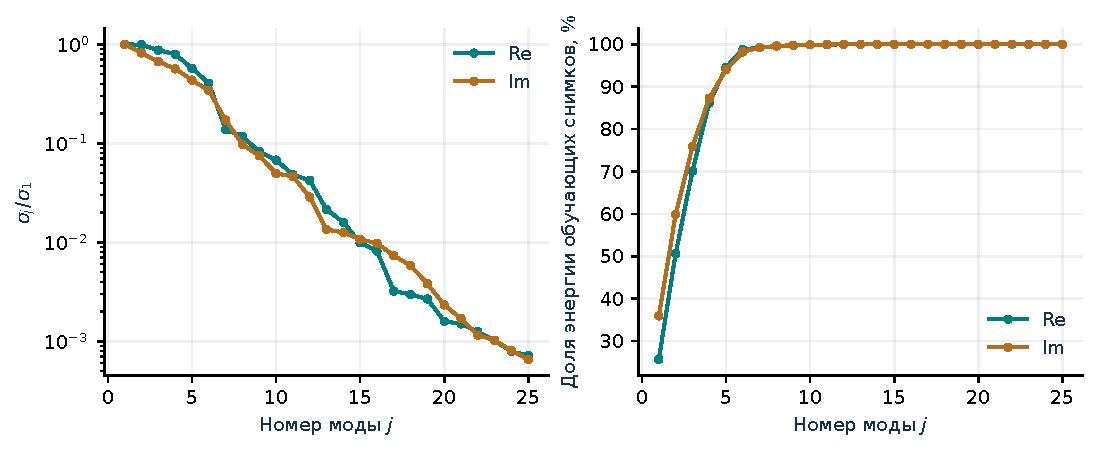
\includegraphics[width=.79\textwidth]{assets/spectrum.pdf}
\caption{Слева --- отношение $\sigma_j/\sigma_1$ в логарифмической шкале.
Справа --- накопленная доля энергии центрированных обучающих полей
в метрике $W$. Показаны сохранённые моды.}
\label{exp:spectrum}
\end{figure}

Числитель доли энергии на рисунке~\ref{exp:spectrum} равен
$\sum_{i=1}^j\sigma_i^2$, а знаменатель --- суммарной
$W$-энергии всех центрированных обучающих полей данного канала.
Для поля из отложенной выборки точность реконструкции проверяют
отдельно по формуле~\eqref{exp:metric}.

\clearpage
\section{Как отделить ошибку базиса от ошибки сети}

Для одного тестового поля сравним три способа получить
коэффициенты одного декодера. Проекция в норме $M$ решает нормальные
уравнения~\eqref{code:consistent-projection} и даёт наименьшую
ошибку для этого поля. Проекция в норме $W$ применяет
POD-кодирование~\eqref{code:pod-encoding}. Обе проекции требуют
значений эталонного поля. Сеть вычисляет коэффициенты по $k$ и
$\theta$, а эталон нужен для оценки прогноза.

\begin{figure}[htbp]
\centering
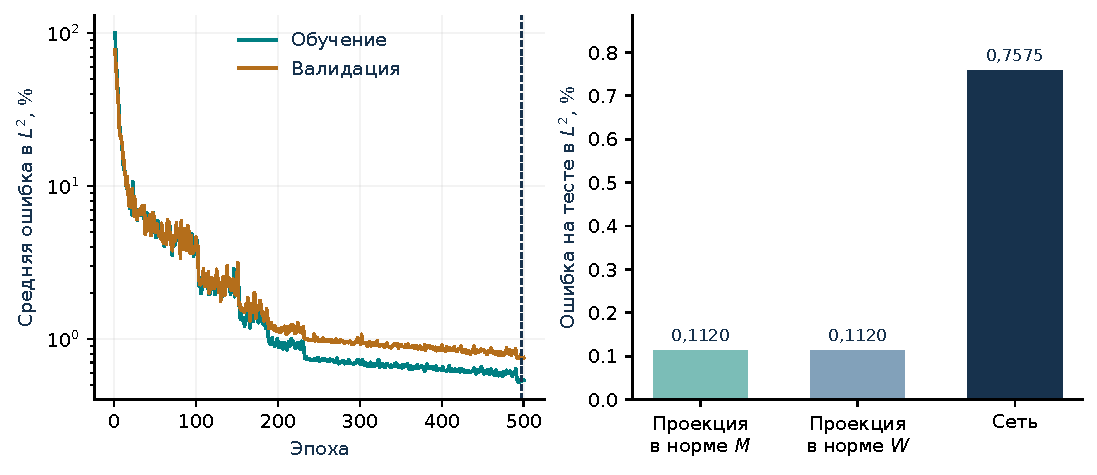
\includegraphics[width=.96\textwidth]{assets/training_and_floor.pdf}
\caption{Слева --- ошибки при обучении SVD-SNO v2 ширины 48,
с шестью блоками и 32\,072 обучаемыми параметрами. Справа ---
средние тестовые ошибки рассеянного поля в норме $M$
для трёх способов получить коэффициенты.}
\label{exp:history}
\end{figure}

На рисунке~\ref{exp:history} кривая «Обучение» усредняет ошибки
мини-пакетов по ходу эпохи. Кривая «Валидация» показывает ошибку с
весами на конец эпохи. При плато валидации шаг оптимизатора
уменьшался вдвое. Обучение дошло до лимита в 500 эпох. Пунктир
отмечает 497-ю эпоху, с которой взяты веса для тестирования.
Ей соответствует минимум валидационной ошибки $0{,}7390\%$.

Обе проекции в среднем дают $0{,}1120\%$ при округлении до четырёх
знаков после запятой. Сеть с тем же декодером даёт $0{,}7575\%$.

\begin{worked}{Какой выигрыш допускает фиксированный декодер?}
Можно ли получить среднюю ошибку $0{,}1\%$ на этих же тестовых
полях, улучшая лишь предсказание коэффициентов?

\textbf{Решение.} Оптимальная проекция эталонных полей даёт в среднем
$0{,}1120\%$. Этот минимум выше цели $0{,}1\%$, поэтому для неё
потребуется изменить пространство декодера. Разность между ошибкой сети
и минимумом составляет около $0{,}6455$ процентного пункта. Это разность
средних ошибок поля. Ортогональное сложение квадратов применяют
к каждому полю отдельно по формуле~\eqref{rig:projection-identity}.
\end{worked}

\clearpage
\section{Как читать карту одного прогноза}

На рисунке~\ref{exp:fields} показан тестовый снимок с ошибкой,
ближайшей к медиане. Его индекс в исходном наборе --- 940,
$k\approx1{,}48616$, $\theta\approx3{,}30401$ рад.
Относительная ошибка рассеянного поля составляет $0{,}3924\%$
с тем же округлением, что и в таблице~\ref{exp:stats}.

\begin{minipage}{\linewidth}
\centering
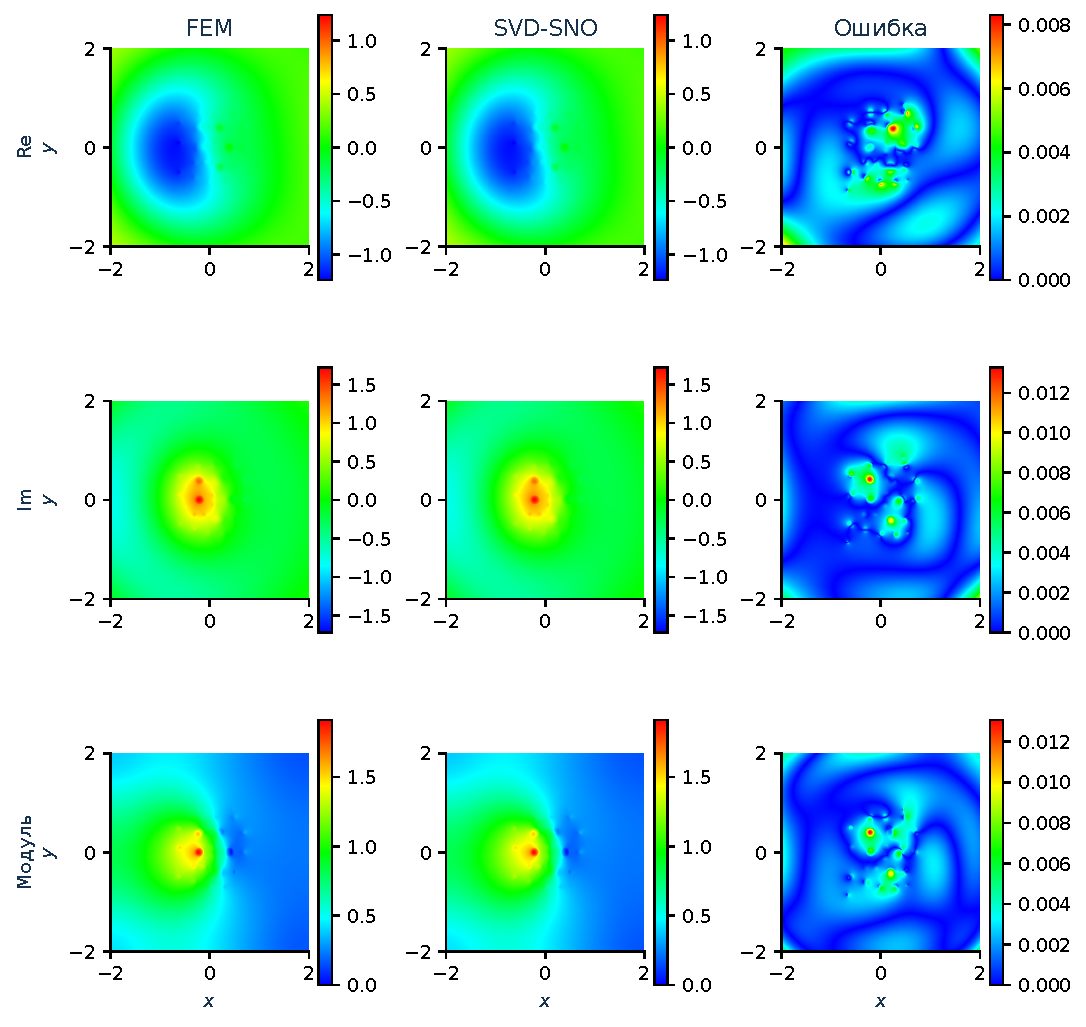
\includegraphics[width=.87\textwidth,height=.58\textheight,keepaspectratio]{assets/field_comparison.pdf}
\captionsetup{hypcap=false}\captionof{figure}{Рассеянное поле по МКЭ (FEM),
прогноз SVD-SNO и абсолютная ошибка. В каждом ряду поле и прогноз даны
в одной шкале, ошибка --- в собственной. Нуль на картах Re и Im поля и прогноза
выделен зелёным, на картах модуля и всех ошибок --- синим.}
\label{exp:fields}
\end{minipage}

Справа в первых двух строках показаны
$|\operatorname{Re}(\widehat u_s-u_{s,h})|$ и
$|\operatorname{Im}(\widehat u_s-u_{s,h})|$. Внизу справа показана
абсолютная разность модулей $\bigl||\widehat u_s|-|u_{s,h}|\bigr|$.
Внутри треугольника цвет определяется по линейной интерполяции узловых значений каждой карты.
Равенство модулей допускает ошибку фазы. Например, при
$\widehat u_s=-u_{s,h}$ нижняя правая карта всюду равна нулю,
а формула~\eqref{exp:metric} для ненулевого поля даёт $200\%$.

\clearpage
\section{Сравнение с GMsFEM на общих запросах}

Все методы в таблице~\ref{exp:comparison} проверены на одних и тех же
216 парах $(k,\theta)$. Рассеянные поля каждого метода вычисляют из
их собственных P1-представлений в точках семиточечной квадратуры
Дюнавана на эталонной сетке. К ним добавляют аналитическую падающую
волну~\eqref{math:incident}, чтобы получить полные поля.
Одна и та же падающая волна сокращается в разности, поэтому числитель
относительной комплексной ошибки совпадает для обоих полей.
Знаменатель берут отдельно для каждого эталона, $u_{s,h}$ и $u_i+u_{s,h}$.

\begin{table}[htbp]
\centering
\caption{Относительная комплексная $L^2$-ошибка в процентах
на общей квадратуре. Эталон --- FEM при $h=0{,}02$.}
\label{exp:comparison}
\begin{tabular}{@{}lrrrr@{}}
\toprule
 & \multicolumn{2}{c}{Рассеянное поле} & \multicolumn{2}{c}{Полное поле}\\
\cmidrule(lr){2--3}\cmidrule(l){4--5}
Метод & Среднее & 95-й перц. & Среднее & 95-й перц.\\
\midrule
SVD-SNO \texttt{low} & $0{,}7575$ & $2{,}6427$ & $0{,}3325$ & $1{,}1946$\\
FEM, $h=0{,}04$ & $0{,}1354$ & $0{,}3301$ & $0{,}0662$ & $0{,}2747$\\
GMsFEM $10\times10$, тип 1 & $3{,}1939$ & $11{,}6721$ & $1{,}9166$ & $9{,}7779$\\
GMsFEM $10\times10$, тип 2 & $1{,}4521$ & $4{,}2627$ & $0{,}7638$ & $3{,}6293$\\
GMsFEM $20\times20$, тип 1 & $1{,}7069$ & $6{,}6413$ & $1{,}0583$ & $5{,}5637$\\
GMsFEM $20\times20$, тип 2 & $0{,}5190$ & $1{,}2992$ & $0{,}2534$ & $1{,}1011$\\
\bottomrule
\end{tabular}
\end{table}

В этом тесте у GMsFEM $20\times20$ типа 2 ниже средние ошибки обоих
полей, чем у SVD-SNO. В каждой конфигурации GMsFEM использовано
по 16 локальных мод на вершину грубой сетки. Для каждого запроса метод
решает редуцированную физическую систему. SVD-SNO предсказывает
коэффициенты 25 глобальных мод в каждой компоненте. Поэтому число мод
означает разное для двух способов реконструкции.

В ошибку GMsFEM относительно эталона входят редукция и различие сеток.
Строка FEM при $h=0{,}04$ показывает межсеточную разницу после решения
полной системы на исходной сетке GMsFEM. Вычитание её
средней ошибки из ошибки GMsFEM даёт разность двух статистик,
а вклад редукции можно измерить прямым сравнением двух полей при
$h=0{,}04$.

\clearpage
\section{Что проверять при большой ошибке}

Обозначим через $u_s$ решение непрерывной задачи с поглощающим
условием, через $u_{s,h}$ --- его FEM-приближение, а через $u_*$ ---
проекцию $u_{s,h}$ в пространство декодера по норме $M$. Для
прогноза $\widehat u_s$ имеем
\[
 u_s-\widehat u_s
 =(u_s-u_{s,h})+(u_{s,h}-u_*)+(u_*-\widehat u_s).
\]
Первое слагаемое проверяют при уточнении FEM-сетки, сравнивая поля
в общих физических точках. Второе измеряют проекцией проверочных
FEM-полей в декодер. Третье измеряют сравнением прогноза с этой же
проекцией. При большом разрыве между ошибкой проекции и ошибкой
сети стоит проверить входные признаки, обратную нормировку
коэффициентов и порядок узлов при декодировании.

Два последних слагаемых ортогональны в норме $M$. Для оценки ошибки
относительно непрерывного решения требуется отдельно оценить
$u_s-u_{s,h}$. Измеренное сравнение двух сеток показывает изменение
FEM-решения между $h=0{,}04$ и $h=0{,}02$. Точность поглощающего
условия и перенос на новые среды требуют отдельных проверок.

Числа для SVD-SNO взяты из
\path{experiments/reference_sno_gmsfem/results/low/sno_metrics.json},
межсеточное сравнение --- из
\path{experiments/reference_sno_gmsfem/results/REPORT.md}.
Параметры показанного поля и происхождение измерений собраны в
\path{svd_sno_manual/assets/evidence.json}.
